\documentclass[../main.tex]{subfiles}
\begin{document}

\chapter{Flows around a topography}
\label{chap:FLOWS}

The first chapter is devoted to the specification and description of the studied problem. Its structure is as follows

\begin{compactenum}
	\item important phenomena associated with orographic flows are described in \Cref{sec:PHENOMENA};
	\item equations governing the flow are formulated in \Cref{sec:GOV-EQUATIONS};
	\item a more detailed description of mountain waves is carried out in \Cref{sec:MTN-WVS};
\end{compactenum}

\todo{SPLIT MATHS AND PHYSICS?}

\section{Physical description}
\label{sec:PHYSICS}

Let us begin by describing orographic flows from the point of physics, providing not only further motivation, but also significant physical aspects of the studied problem.

\subsection{Observed phenomena}
\label{sec:PHENOMENA}

\subsubsection{Internal gravity waves}
\label{sec:internal-gws}

\emph{Internal gravity wave}: is a type of wave phenomenon arising under certain (although common) atmospheric conditions\sidenote{More detail on these conditions is given in the section \Cref{chap:FLOWS}.}. Orographic flows typically induce two types of internal gravity waves: \emph{mountain waves} and \emph{lee waves} \autocite[p.~60]{nappoIntroductionAtmosphericGravity2013}. Although IGWs generated by a flow over terrain influence mainly the dynamics of atmosphere locally near that terrain, their contribution \emph{cannot be neglected} also in global climate and weather forecasts, due to the energy transfer across layers of the atmosphere that is typical for gravity waves \autocite[p.~58]{nappoIntroductionAtmosphericGravity2013}.

\begin{figure}[htbp]
	
\includegraphics[width=\linewidth]{clouds}
	\caption{Lenticular clouds formed under the influence of mountain waves.}
	\floatfoot{Source: \autocite{joiseyshowaaLenticularCloudsIceland2018}}
	\label{fig:clouds}
\end{figure}


\subsubsection{Downslope windstorms}
\label{sec:downslope-windstorms}

Under specific physical conditions\sidenote{To be transparent, it should be noted that the model of orographic flow under our study is \emph{unable} to describe downslope windstorms on its own, as it deals only with \emph{dry air.} The physics responsible for the emergence of downslope windstorms is the difference between \emph{dry} and \emph{moist} adiabatic lapse rates. Nevertheless, our model is capable of capturing mountain waves that interfere with downslope windstorms.}, air carried by a flow over a mountain obstacle can arrive warmer and drier at the lee side of the mountain, manifesting as \emph{warm} gusts of air descending from mountains into valleys. These types of winds are called \begin{inparaenum} \item chinook in North America; \item f\"ohn in Europe. \end{inparaenum} 
The interference of such winds with mountain \textcolor{gray}{and lee} waves can manifest as gusts of hurricane-level force \autocite[p.~307]{sutherlandInternalGravityWaves2010}, posing a great threat to the inhabitants and infrastructure of nearby regions.

\begin{figure}[htbp]
	
\includegraphics[width=\linewidth]{fohn}
	\caption{Downslope windstorm in Valle de Losa, Castile and León}
\floatfoot{Source: \autocite{varelaEfectoFoehnFohn2013}}
	\label{fig:downslope-windstorm}
\end{figure}

\subsubsection{Clear-air turbulence}
\label{sec:CAT}
As mentioned, IGWs serve as an important mechanism of energy transfer across layers of the atmosphere. If particular conditions are met, it can happen that the wave propagating upwards grows in amplitude. Breakdown of these waves can produce a specific kind of turbulence, the so called \emph{clear-air turbulance.} This turbulence is extremely dangerous to aerial transport, as its presence is not accompanied by any kind of visual effects, hence the name \autocite[p.~58]{nappoIntroductionAtmosphericGravity2013}. A model that accurately captures mountain waves \emph{could} be helpful in predicting areas of CAT.

\todo{FIGURES}

\subsection{Governing equations}
\label{sec:GOV-EQUATIONS}

The crucial part about consistent mathematical modelling of physical processes is deciding \emph{which equations to solve.} The atmospheric science community adopts various models ranging in complexity and the amount of physical phenomena it is able to capture: one could be interested in \viz global circulation, cloud microphysics (evaporation, condensation, precipitation), chemical mixing \& transport, radiative processes. In this work, we are interested mostly in \emph{fluid dynamics}, that is the description of the flow.

\subsubsection{Mechanics}
\label{sec:MECHANICS}

Recall the fundamental balance laws governing fluid flows

\begin{description}
	\item[Balance of mass]\mbox{}
	\begin{equations}[single,!,numberline=all]
	\label{eq:MASS-BALANCE}
	\tdot{\rho} + \rho \div \vb{v} = 0 \eqcomma
	\end{equations}
	\item[Balance of linear momentum]\mbox{}
	\begin{equations}[single,!,numberline=all]
	\label{eq:MOMENTUM-BALANCE}
	\rho \tdot{\vb{v}} = \div \cstress + \rho \vb{b} \eqend
	\end{equations}
\end{description}

In \Cref{eq:MASS-BALANCE}, \Cref{eq:MOMENTUM-BALANCE} $\vb{v}$ is the velocity field, $\rho$ is the \textcolor{gray}{mass} density, $\cstress$ is the Cauchy stress tensor and $\vb{b}$ is the \textcolor{gray}{specific} density of body forces. The dot operator stands for the material (convective) time derivative, that is 

\begin{equations}[single,*]
	\tdot{\varphi} = \begin{cases} \partial_t \varphi & \text{in the Lagrangian frame,} \\ \partial_t \varphi + \vb{v} \cdot \grad \varphi & \text{in the Eulerian frame.} \end{cases}
\end{equations} 


To close the system, a constitutive relation for the Cauchy stress tensor has to be provided.\sidenote{As well as boundary and initial conditions; these will be discussed in \Cref{sec:IBCONDITIONS}.} The fluid of our interest is \emph{air}, which is commonly modelled as an \emph{inviscid compressible Newtonian fluid}, for which\sidenote{In the case of compressible Newtonian fluids, a general constitutive closure for the Cauchy stress tensor reads as \begin{equations}[single,*]
\cstress = -p \identityM + \lambda \left(\div \vb{v}\right)\identityM + 2 \mu \symvgrad,
\end{equations}
where $\symvgrad = \sym \grad \vb{v}$ and $\lambda, \mu$ being the viscosity coefficients. More precisely, $\mu$ is the \emph{shear viscosity} and $\lambda$ contributes to the \emph{bulk viscosity} $\zeta = \frac{3 \lambda + 2 \mu}{3}$. In the case of an \emph{inviscid} fluid, we put $\mu = 0 = \zeta,$ \ie the fluid does not pose any resistance to shear deformation nor compression/expansion.}

\begin{equations}[single,!,numberline=all]
\label{eq:CAUCHY}
\cstress = - p \identityM,
\end{equations}

where $p$ is the thermodynamic pressure and $\identityM$ is the identity matrix. This constitutive asumption is standard in the field of internal gravity waves modelling \autocite{teixeiraPhysicsOrographicGravity2014,smithInfluenceMountainsAtmosphere1979,frittsGravityWaveDynamics2003,doyleIntercomparisonTREXMountainwave2011}. 

While it is standard to neglect bulk and shear viscosity, \ie the \emph{molecular viscosity}, some attention should be payed to turbulence and the \textcolor{gray}{effective} \emph{eddy viscosity} frequently used in its modelling \autocite[p.~5]{smagorinskyGENERALCIRCULATIONEXPERIMENTS1963}\autocite[p.~93]{popeTurbulentFlows2000}. At this point, a second important distinction should be made: not only are we interested in the flow solitarily, \emph{we declare internal gravity waves to be our main interest.} When dealing with internal gravity waves however, the Reynolds number of the flow is so great that even the effective eddy viscous forces are unimportant \autocite[p.~30]{sutherlandInternalGravityWaves2010}. Hence, ultimately we do not assume \begin{inparaenum} \item any kind of \textcolor{gray}{physical} viscosity\sidenotemark, \item turbulence parametrization. \end{inparaenum} \sidenotetext{The used discretization schemes however deploy some \emph{numerical} viscosity -- a standard stabilization technique.}

Finally, let us address the body forces $\vb{b}.$ In middle atmosphere dynamics, there are usually two main contributions: \begin{inparaenum} \item the Earth's gravity $\vb{g}$ \item Coriolis force \end{inparaenum}. Within our work, we \emph{neglect} the Coriolis force, and thus only assume the gravity; a discussion on the effects of the Coriolis force on internal gravity waves can be found in\autocite[p.~206]{sutherlandInternalGravityWaves2010}.

With the form of the Cauchy stress tensor \Cref{eq:CAUCHY} and the simplified assumption of present body forces the balance of momentum \Cref{eq:MOMENTUM-BALANCE} hence reads as

\begin{equations}[single,!,numberline=all]
\label{eq:MOMENTUM_EQ}
\rho \tdot{\vb{v}} = - \grad p + \rho \vb{g},
\end{equations}

where $p$ is the \emph{thermodynamic} pressure. 

\subsubsection{Thermodynamics}
\label{sec:THERMODYNAMICS}

Our balance laws \Cref{eq:MOMENTUM-BALANCE}, \Cref{eq:MOMENTUM_EQ} have been formulated for a general inviscid compressible Newtonian fluid. To specify the continuous media of our interest, one has to specify the \emph{equations of state}, in particular provide a relation for the pressure $p$ and for the \textcolor{gray}{specific density of} internal energy $e$. As stated previously, the amount of attention we wish to pay to thermodynamics is limited, and as such we restrict ourselves to the thermodynamics of an ideal gas:

\begin{description}
	\item[Thermal equation of state]\mbox{}
	\begin{equations}[single,!,numberline=all]
	\label{eq:THERMAL}
	p\left(\rho, T\right) = R \rho T,
	\end{equations}
	\item[Caloric equation of state]\mbox{}
	\begin{equations}[single,!,numberline=all]
	\label{eq:CALORIC}
	e\left(\rho, T\right) = c_V T,
	\end{equations}
	\item[Entropy equation]\mbox{}
	\begin{equations}[single,!,numberline=all]
	\label{eq:ENTROPY}
	\eta\left(\rho, T\right) = \eta_{\text{ref}} + c_V \log\left(\frac{R T}{\rho^{\gamma - 1}}\right).
	\end{equations}
\end{description}

In the above equations, $T$ is the thermodynamic temperature, $R$ is the specific gas constant, $c_V$ is the specific heat at constant volume per unit mass, $\eta_{\text{ref}}$ is the reference value of \textcolor{gray}{the specific density of} entropy, $\gamma$ is the Poisson ratio. For dry air the values of these approximately are $R = \qty{287}{\joule \kilogram^{-1} \kelvin^{-1}}, c_V = \qty{717}{\joule \kilogram^{-1} \kelvin^{-1}}, \gamma = \frac{7}{5}.$

\subsubsection{Potential temperature}
\label{sec:POTENTIAL_TEMP}

In continuum thermodynamics of fluids, it is generally convenient to describe thermodynamic states using the density $\rho$ and \emph{thermodynamic} temperature $T$. In atmospheric sciences, it is common (and not entirely unphysical) to assume some processes to be \emph{adiabatic} or more precisely, \emph{isentropic} (meaning that they are adiabatic and also \emph{reversible}.) \sidenote{Although a simplification, the assumption of adiabaticity allows explaining various phenomena including \viz \begin{compactitem}
	\item downslope windstorms;
	\item katabatic winds;
	\item propagation of acoustic waves. 
\end{compactitem}
}

In such cases, it is convenient to introduce a \emph{conservative} thermodynamic variable -- \emph{potential} temperature $\theta$; let us introduce it now.
Consider a fluid in a thermodynamic state $(T, p)$ described by temperature $T$ and pressure $p$ that undergoes isentropic evolution to the state $(\theta, p_0).$ Then from \Cref{eq:ENTROPY} it follows

\begin{equations}[single,*]
\eta_{\text{ref}} + c_V \log\left(\frac{R T}{\rho^{\gamma - 1}}\right) = \eta_{\text{ref}} + c_V \log\left(\frac{R \theta}{\rho_0^{\gamma-1}}\right),
\end{equations}

and so

\begin{equations}[single,*]
\frac{T}{\rho^{\gamma-1}} = \frac{\theta}{\rho_0^{\gamma-1}}.
\end{equations}

Expressing now $\theta$ with the aid of the definition of the Poisson ratio $\gamma = \frac{c_p}{c_V}$, with $c_p$ being the specific heat at constant pressure per unit mass, and the Mayer relation $c_p - c_V = R$ one obtains

\begin{equations}[single,*]
\theta = T\left(\frac{\rho_0}{\rho}\right)^{\gamma - 1} = T\left(\frac{\rho_0}{\rho}\right)^{\frac{R}{c_V}} = T\left(\frac{p_0}{R \theta} \frac{R T}{p}\right)^{\gamma -1},
\end{equations}

where we have used the thermal equation of state \Cref{eq:THERMAL} $p_0 = R \rho_0 \theta.$ Solving for $\theta$ now gives

\begin{equations}[single,*]
\theta = T \left(\frac{p_0}{p}\right)^{\frac{\gamma - 1}{\gamma}},
\end{equations}

and since $\frac{\gamma -1}{\gamma} = \frac{c_p - c_V}{c_V} \frac{c_V}{c_p} = \frac{R}{c_V} \frac{c_V}{c_p} = \frac{R}{c_p},$ we have arrived at a common expression

\begin{equations}[single,!,numberline=all]
\label{eq:POTENTIAL}
\theta = T\left(\frac{p_0}{p}\right)^{\frac{R}{c_p}}.
\end{equations}

The quantity $\theta$ is called the \emph{potential temperature}. Let us summarize its meaning: it is the thermodynamic temperature an ideal gas (like \emph{dry air}) would possess if \emph{adiabatically} moved from the thermodynamic state $(T, p)$ to the state $(\theta, p_0).$ In meteorological context, the reference pressure $p_0$ is always taken to be $p_0 = \qty{1013.25}{\hecto \pascal},$ \ie atmospheric pressure at sea level. Potential temperature is especially useful, since it is \emph{conserved} under \emph{isentropic flows}. Indeed, under the isentropic constraint from \Cref{eq:ENTROPY} it follows

\begin{equations}[single,*]
	\text{const} \, = \eta =  \eta_{\text{ref}} + c_V \log\left(\frac{R \theta}{\rho^{\gamma-1}}\right),
\end{equations}

and so 

\begin{equations}[single,*]
	\theta = \frac{\rho_0^{\gamma - 1}}{R}\exp\left(\frac{\eta - \eta_{\text{ref}}}{c_V}\right).
\end{equations}

The right-hand side contains only constants, so we see

\begin{equations}[single,!,numberline=all]
\label{eq:THETA-CONSTANT}
\theta = \, \text{const},
\end{equations}

and in particular

\begin{equations}[single,!,numberline=all]
\label{eq:THETA-ADVECTED}
\tdot{\theta} = 0.
\end{equations}

\emph{Under isentropic flows, $\theta$ is conserved.}

\subsubsection{Complete system }
\label{sec:SYSTEM}
Let us summarize the governing equations, describing \emph{solely} the flow of inviscid dry air

\begin{equations}[columns,!,numberline=all]
\label{eq:GOVERNING-SYSTEM}
\dot{\rho} + \rho \div \vb{v} &= 0, \\
\rho \tdot{\vb{v}} &= - \grad p + \rho \vb{g}, \\
\tdot{\theta} &= 0,\\
p(\rho, T) &= R \rho T.
\end{equations}


\subsubsection{Hydrostatic balance}
\label{sec:HYDROSTATICS}

Let us look for \emph{stationary solutions of} the system \Cref{eq:GOVERNING-SYSTEM}. Choosing an inertial frame of reference $\left(\vb{e}_x, \vb{e}_z\right)$ such that $\vb{g} = g \vb{e}_z$ and denoting $\vb{v} = u \vb{e}_x + w \vb{e}_z$.

\subsection{Mountain waves}
\label{sec:MTN-WVS}

\subsubsection{Stratification}
\label{sec:STRATIFICATION}

\subsubsection{Buoyancy oscillations }
\label{sec:BUOYANCY}

When an air parcel hits a mountain barrier, the topography can act as a ramp and eject the air parcel into higher altitude. In the case of a \emph{stably stratified atmosphere}, the buoyancy force decreases with altitude, and thus the net force acting on the air parcel points downwards. On its way to lower altitude, the air parcel overshoots its equilibrium position, which in turn leads to the \emph{increase} of buoyancy force, resulting in a total acceleration pointing upwards. This buoyancy-driven oscillatory motion can be thought of as a prototype of an \emph{internal gravity wave}. When the initial displacement from the equilibrium state of the air parcel is caused by a flow over topography, the resulting gravity wave is called \emph{a mountain wave.} \autocite[p.~143]{sutherlandInternalGravityWaves2010} A different type of gravity waves associated with orographic flows are \emph{lee waves}: gravity waves trapped between the ground and upper levels of the atmosphere due to reflection \autocite[p.~60]{nappoIntroductionAtmosphericGravity2013}.

\begin{figure}[htbp]
	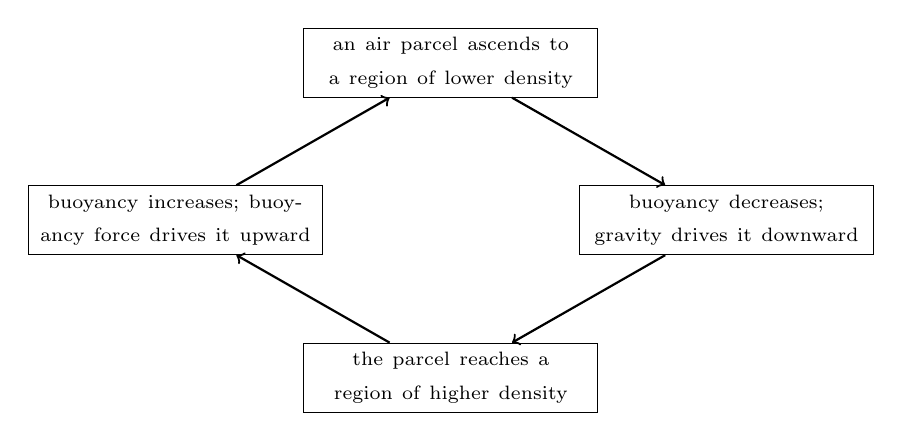
\begin{tikzpicture}[node distance = 2cm]
		\node (A) [draw, align=center, text width=3.5cm] at (0,2) {\scriptsize an air parcel ascends to a region of lower density};
		\node (B) [draw, align=center, text width=3.5cm] at (3.5,0) {\scriptsize buoyancy decreases; gravity drives it downward};
		\node (C) [draw, align=center, text width=3.5cm] at (0,-2) {\scriptsize the parcel reaches a region of higher density};
		\node (D) [draw, align=center, text width=3.5cm] at (-3.5,0) {\scriptsize buoyancy increases; buoyancy force drives it upward};
		\draw[->,thick] (A) -- (B);
		\draw[->,thick] (B) -- (C);
		\draw[->,thick] (C) -- (D);
		\draw[->,thick] (D) -- (A);
	\end{tikzpicture}
	\caption{Buoyancy oscillation prototype}
	\label{fig:GW-diagram}
\end{figure}

\subsubsection{Linear wave theory}
\label{sec:LINEAR-THEORY}

\begin{figure}[htbp]
	\centering
	\begin{tikzpicture}[
		>={Stealth[length=2.5mm]},
		wave/.style = {thick},
		flow/.style = {-Stealth, thick},
		pert/.style = {-{Stealth[length=2mm]}, semithick},
		]
		% ---- parameters -------------------------------------------------
		\def\A{0.5}          % wave amplitude
		% wavelength = 4 units: sin(90*x) has period 360/90 = 4
		\def\xmin{-0.3}
		\def\xmax{10.3}      % ~2.5 periods

		% ---- corrugated surface -----------------------------------------
		\draw[wave, samples=200, smooth, domain=\xmin:\xmax]
		plot (\x, {\A*sin(90*\x)});

		% ---- freestream arrow -------------------------------------------
		\draw[flow] (1.0, 2.0) -- node[above] {$u_0$} ++(2.0, 0);

		% ---- anchor points on the first period --------------------------
		%   crest at x=1, zero-descend at x=2, trough at x=3
		\coordinate (rise)  at (0.4, {\A*sin(90*0.4)});  % mid-ascent
		\coordinate (crest) at (1.0, \A);
		\coordinate (fall)  at (1.6, {\A*sin(90*1.6)});  % mid-descent

		% ---- labels on the first period ---------------------------------
		\node[align=center, anchor=south east]
		at ($(rise) + (-0.05, 0.15)$)
		{$\theta_1 < 0$ \\ $p_1 < 0$ \\ $u_0 - u_1$};

		\node[align=center, anchor=south]
		at ($(crest) + (0, 0.15)$)
		{$w_1 = 0$ \\ $u_1 = 0$};

		\node[align=center, anchor=south west]
		at ($(fall) + (0.05, 0.15)$)
		{$\theta_1 > 0$ \\ $p_1 > 0$ \\ $u_0 + u_1$};

		% parcel-velocity arrows along the slopes
		\draw[pert] ($(rise) + (-0.3,-0.15)$) -- ($(rise) + ( 0.15, 0.30)$);
		\draw[pert] ($(fall) + (-0.15, 0.30)$) -- ($(fall) + ( 0.30,-0.15)$);

		% ---- perturbation components at later phases --------------------
		% descending zero at x=6: u_1 > 0, w_1 < 0
		\coordinate (pA) at (6, 0);
		\draw[pert] (pA) -- ++( 0.6, 0   ) node[right] {$u_1$};
		\draw[pert] (pA) -- ++( 0,  -0.6 ) node[below] {$w_1$};

		% ascending zero at x=8: u_1 < 0, w_1 > 0
		\coordinate (pB) at (8, 0);
		\draw[pert] (pB) -- ++(-0.6, 0  ) node[left]  {$u_1$};
		\draw[pert] (pB) -- ++( 0,   0.6) node[above] {$w_1$};
	\end{tikzpicture}
	\caption{Variations of wave-perturbation quantities along a surface corrugation.}
	\label{fig:surface-corrugation}
\end{figure}

\end{document}

